%% IEICE Technical Report (ieicej.cls) - dense 8-page version without external figs
%% NOTE: This class requires pLaTeX/uplatex workflow (DVI -> PDF).

\documentclass[technicalreport]{ieicej}
\usepackage[dvipdfmx]{graphicx}

\usepackage[fleqn]{amsmath}
\usepackage{newtxtext}
\usepackage[varg]{newtxmath}
\usepackage{url}

\urlstyle{rm}

% ===== Optional macros =====
\newcommand{\LLM}{LLM}
\newcommand{\GCN}{GCN}

% ===== Metadata =====
\tecrepyear{2026}
\titlepagebaselinestretch{0.88}

\jtitle{路線図・気象情報を統合した \LLM\ Agent による鉄道旅客数変動の説明生成枠組み}
\etitle{Explaining Railway Passenger Fluctuations: An \LLM\ Agent Framework Integrating Route and Weather Data}

\authorlist{%
 \authorentry{成瀬 宥哉}{Yuya NARUSE}{Oita}
 \authorentry{大知 正直}{Masanao OCHI}{Oita}
}

\affiliate[Oita]{大分大学 理工学部 共創理工学科 知能情報システムコース}
{Oita University, Faculty of Science and Technology, Intelligent Information Systems Course}

\begin{document}

\begin{jabstract}
鉄道の旅客需要予測は，ダイヤ設定，混雑緩和，輸送力配分などの運用判断を支援する上で重要である。しかし，現場では予測値のみでは不十分であり，旅客数の増減がなぜ生じたのかを，運用担当者が理解可能な形で提示することが求められる。特に，鉄道需要の変動は降雨・気温等の気象条件と，隣接駅・乗換駅を介した駅間波及が重畳して生じるため，単一駅の時系列のみから原因を説明することは難しい。既存研究では，\GCN\ 等により駅間依存を考慮した予測精度向上が進んでいる一方，外部根拠と駅間依存を統合し，旅客数の増減要因を自然言語で根拠付きに説明する枠組みは十分に整備されていない。そこで本研究では，路線図と時系列共変動に基づく機能的フローネットワークを構築し，\GCN\ により駅間依存を考慮した需要推定を行う。さらに，降雨量・気温等の気象特徴量と近傍駅変動の要約統計を入力として \LLM\ Agent を動作させ，増減要因を根拠とともに記述した説明レポートを生成する。評価では，要因の正解ラベルを付与可能な模擬データを用いて，気象要因および駅間波及に関する説明の妥当性を定量評価した。その結果，気象情報の統合により原因推測成立率が76.7ポイント，パターン一致度が43.8ポイント改善し，駅間波及情報の統合により近接駅由来の説明一致度が100ポイント向上した。また，\GCN\ により需要推定誤差（MSE）が0.3111から0.2703へ改善し，駅間依存を考慮する有効性を確認した。以上より，運用担当者が参照可能な根拠を明示しつつ説明を生成する枠組みの有用性を示した。
\end{jabstract}

\begin{jkeyword}
LLM，LLM Agent，グラフ畳み込みネットワーク，交通需要予測，説明生成
\end{jkeyword}

\begin{eabstract}
Railway passenger demand forecasting supports operational decisions such as timetable planning, congestion mitigation, and capacity allocation. However, numerical forecasts alone are insufficient in practice because operators must understand why passenger demand increases or decreases. Demand fluctuations are caused not only by external factors such as weather conditions but also by propagation effects through neighboring and transfer stations, making it difficult to explain the reasons from a single-station time series alone. Although previous studies have improved forecasting accuracy by incorporating inter-station dependencies with graph-based models such as Graph Convolutional Networks (\GCN), a framework that integrates both external evidence and network dependencies to generate grounded natural-language explanations has not been sufficiently established. In this study, we propose an integrated framework that combines a functional flow network, demand estimation with \GCN, and explanation generation by an \LLM\ Agent. The proposed method constructs a graph from railway connections and co-movement patterns among stations, and estimates short-term passenger demand while considering inter-station dependencies. Weather features such as rainfall and temperature, together with summarized neighboring-station changes, are then fed into the \LLM\ Agent to generate explanatory reports describing the causes of demand increases or decreases. Experiments using simulated data with ground-truth labels showed that integrating weather information improved the causal inference success rate by 76.7 points and pattern matching by 43.8 points, while integrating propagation information improved neighboring-station explanation accuracy by 100 points. In addition, incorporating inter-station dependencies through \GCN\ improved the MSE from 0.3111 to 0.2703. These results suggest the practical usefulness of generating grounded explanations that explicitly present operationally interpretable evidence.
\end{eabstract}

\begin{ekeyword}
LLM, LLM Agent, GCN, passenger demand, explanation generation
\end{ekeyword}

\maketitle

\section{まえがき}
都市鉄道の運用では，短期的な旅客需要予測に基づいてダイヤ調整や要員配置を行う。しかし，実運用においては予測値そのものだけでなく，「なぜ増えたのか」「なぜ減ったのか」という理由の把握が重要である。特に，降雨や高温といった外部要因と，隣接駅・乗換駅を介した需要変動の波及が重なる場合，数値予測のみから原因を即時に説明することは難しい。

近年，交通系ICカード乗降データの蓄積により，駅単位・時間単位での高精細な需要観測が可能となった。これに伴い，RNN，LSTM，Transformer，時空間GNNなどを用いた需要予測研究が進展している。一方で，予測モデルが高精度化するほど内部構造が複雑となり，現場で理解可能な形で根拠を提示することは困難になりやすい。また，\LLM\ による説明生成が注目されているが，鉄道固有の駅間依存や当日の外部要因と整合した説明を常に生成できるとは限らない。

そこで本研究では，気象要因と駅間依存を明示的な根拠として扱い，\GCN\ による需要推定と \LLM\ Agent による説明生成を統合した枠組みを提案する。

\section{関連研究}
本研究は，ICカード乗降データを対象に，気象要因と駅間依存を統合し，\GCN\ による需要推定と \LLM\ Agent による根拠付き説明生成を一体化する枠組みを提案する。このため関連研究は時系列予測モデル，時空間GNN，データ駆動型グラフ学習，外生要因統合，説明可能AIおよび \LLM\ の活用，の観点から整理する。

まず，交通需要予測の基盤として，RNNやLSTMに代表される系列モデルが広く用いられてきた。LSTMは長期依存の学習困難を緩和する構造として知られており，時系列予測タスクにおける有効性が多く報告されている。さらに，Transformerは自己注意機構により系列内の長距離依存を並列的に扱う枠組みを確立し，時系列分析にも応用されている。しかし，鉄道需要のように観測点がネットワーク構造を持つ問題では，時間依存だけでなく，駅間の関係性を明示的に扱う必要がある。

この課題に対し，交通分野では時空間GNNが主流となってきた。グラフ学習の基礎として，\GCN\ による半教師あり学習の枠組みや，局所化スペクトルフィルタリングによる効率的なグラフ畳み込みが提案されている。交通予測の代表例として，DCRNNは拡散畳み込みと系列モデルを組み合わせて交通流の方向性を表現し，STGCNは時空間畳み込みにより高い予測性能を示している。さらに，AST-GCNは属性情報を組み込み，外部情報を含む予測の有効性を示している。これらの研究は予測精度向上において重要であるが，出力結果を自然言語で説明することまでは直接扱っていない。

また，駅間依存を与えるグラフ構造についても課題がある。鉄道では，単純な地理隣接だけでは実際の利用関係を十分に表せない場合がある。例えば，乗換駅や都心ターミナル駅では，路線図上で離れた駅同士でも強い需要連動が生じうる。この問題に対し，Graph WaveNetやAGCRNでは，データ駆動型に適応的隣接行列を学習する手法が提案されている。これらは固定グラフに依存しない柔軟な依存関係学習を可能にするが，学習された関係が運用者にとって理解しやすい形で提示されるとは限らない。したがって，本研究では，説明可能性の観点からも共変動に基づく機能的フローネットワークを用い，その近傍情報を \LLM\ に渡す設計を採る。

さらに，交通需要は外生要因の影響を強く受ける。特に降雨，気温，風などの気象条件は公共交通需要に系統的な影響を持つことが報告されている。イベントや祝日等の外部情報を加えることで予測精度を高める研究も存在するが，多くは予測値の改善を主目的としており，なぜその変動が起きたのかを説明するところまでは十分に議論されていない。現場運用では，予測値よりもむしろその背景要因が重要であるため，外生要因統合を説明生成へつなげる設計が必要である。

説明可能性の観点では，注意機構やXAIの利用も議論されている。GATは近傍重みを学習できるため，どのノードが影響したかを示す手がかりになりうるが，注意重みをそのまま因果的根拠とみなすことには慎重さが求められる。また，深層学習モデルの挙動を可視化する手法も提案されているが，鉄道需要の実務で必要とされる「降雨による需要減」「近傍駅からの波及」といったドメイン単位の説明へ自然に落とし込むには限界がある。

近年は \LLM\ を用いた説明可能AIが注目されている。交通流予測に対して \LLM\ による言語説明を付与する研究も報告されており，数値予測を運用者に理解しやすい形へ変換する可能性が示されている。しかし，\LLM\ 単体では一般知識に基づく補完が混入しやすく，観測事実と不整合な説明が生じるリスクがある。このため，\LLM\ を交通需要説明に用いる際には，どの数値事実とどの構造情報を根拠として与えるかを設計する必要がある。

以上より，既存研究では，予測精度向上のための時空間GNN，柔軟な依存関係学習，外生要因統合，\LLM\ による説明生成が個別には進展しているものの，\GCN\ による需要推定結果，気象要因，近傍駅変動を統合し，それらを根拠として自然言語説明を生成し，さらにその妥当性を定量評価する枠組みは十分ではない。本研究はこのギャップを埋めることを目的とする。

\section{提案手法}
\subsection{全体アーキテクチャ}
提案フレームワークは，(1) 入力データ整備，(2) 機能的フローネットワーク構築，(3) \GCN\ による需要推定，(4) \LLM\ Agent による根拠付き説明生成，の4段階から成る。図\ref{fig:overview}に全体像を示す。

\begin{figure}[t]
  \centering
  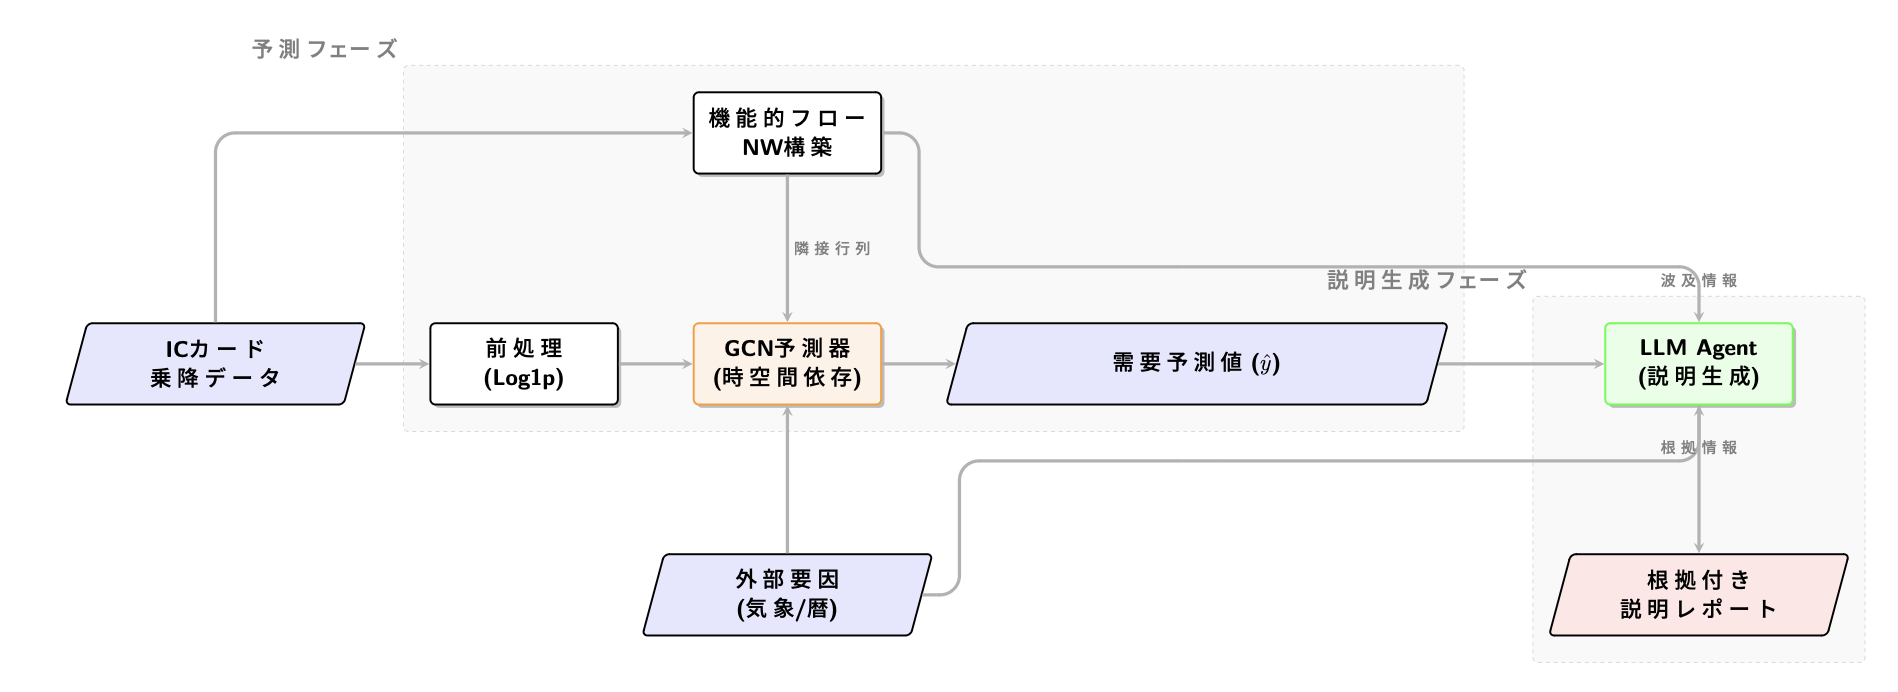
\includegraphics[width=0.90\linewidth]{figs/Architecture.png}
  \caption{提案フレームワークの全体アーキテクチャ}
  \label{fig:overview}
\end{figure}

\subsection{入力データと前処理}
入力として，駅ごとに1時間単位で集計したICカード乗降データを用いる。実験では179時間分のログと1,887駅を対象とした。需要系列の裾の重さを緩和するため，駅$i$，時刻$t$における乗降者数 $x_{i,t}$ に対して次式の対数変換を行う。
\begin{equation}
y_{i,t}=\log(1+x_{i,t})
\label{eq:log1p}
\end{equation}
その後，各駅ごとにZスコア正規化を施し，駅規模の差による支配を抑える。時間情報は時刻・曜日を $\sin,\cos$ による循環特徴量として与え，23時から0時への不連続を回避する。これにより，モデルは絶対規模ではなく増減パターンの類似性に着目しやすくなる。

\subsection{外部要因信号の構成}
外部要因として，降雨量，気温，風速，週末フラグ等を扱う。これらは予測モデルの特徴量として用いるだけでなく，\LLM\ Agent に対して「当該時刻にどの要因が成立しうるか」を示す根拠情報として入力する。説明生成では，単なる数値列ではなく，要因候補として解釈可能な形式に整形し，例えば「降雨あり」「高温条件成立」「近傍駅で直前急増あり」といった入力へ変換する。

\subsection{機能的フローネットワークの構築}
駅間依存は，単純な地理隣接ではなく，共変動に基づく機能的結合として表現する。駅$\times$時間帯行列から駅ペアの類似度を計算し，各駅について相関上位$k$近傍のみを残すことで疎な隣接行列 $A$ を構成する。学習安定化のため，自己ループ付きの対称正規化行列
\begin{equation}
\hat{A}=D^{-1/2}(A+I)D^{-1/2}
\label{eq:adj}
\end{equation}
を用いる。これにより，路線図上の接続だけでなく，利用パターン上の強い結び付きも捉えられる。

\subsection{\GCN\ による需要推定}
需要推定では，時間特徴のみの線形モデル（Linear only）と，\GCN\ 由来の近傍集約特徴を追加したモデル（Linear + GCN-feats）を比較する。\GCN\ は予測器というより，機能的フローネットワーク上で近傍情報を集約する特徴抽出器として利用する。損失関数には，駅平均利用量 $\mu_i$ に基づく重み付きMSEを用いる。
\begin{equation}
L=\frac{1}{T}\sum_{t\in T}\frac{1}{N}\sum_{i=1}^{N} w_i(\hat{y}_{i,t}-y_{i,t})^2,
\quad
w_i=\frac{1}{\sqrt{1+\mu_i}}
\label{eq:wmse}
\end{equation}
これにより，大規模ハブ駅の誤差に学習が過度に引っ張られることを防ぐ。需要予測の精度向上だけでなく，どの近傍が影響しているかという説明の土台も同時に得られる。

\subsection{\LLM\ Agent による根拠付き説明生成}
\LLM\ Agent には，(1) 対象駅・対象時刻の予測増減，(2) 気象状態，(3) 近傍駅の直前変動，を入力する。Agent は，主因が気象要因か，近接駅からの波及かを推論し，根拠を明示した短い説明レポートを生成する。これにより，「降雨により全体需要が低下した」「近接駅の急増が対象駅へ波及した」といった説明を自然言語で提示できる。本研究では，\LLM\ の自由生成をそのまま使うのではなく，許可ラベル集合と候補根拠を与えた上で分類・要約させる構成を採った。

\section{実験}
本章では，提案手法の有効性を，予測性能と説明性能の両面から検証する。評価は三つの観点から行った。第一に，\LLM\ Agent に外部要因を与えることで説明性能が改善するかを確認した。第二に，機能的フローネットワークと \GCN\ により需要推定精度が向上するかを評価した。第三に，気象情報と駅間波及情報の統合が，説明の妥当性にどのように寄与するかをアブレーションで検証した。

\subsection{説明評価用模擬データ}
正解ラベルが既知の評価環境を構築するため，ベース需要 $B_{s,t}$ に対して外部要因の影響を重畳した模擬データを生成した。要因集合を $\mathcal{K}$，要因$k$の影響度を $w_k$，時刻$t$の要因特徴を $x_{k,t}$ とすると，観測需要を次式で与える。
\begin{equation}
y_{s,t}=B_{s,t}\left(1+\sum_{k\in\mathcal{K}}w_kx_{k,t}\right)+\varepsilon_{s,t}
\label{eq:synth}
\end{equation}
ここで $\varepsilon_{s,t}$ は観測ノイズである。これにより，各要因の寄与を既知とした状態で説明性能を評価できる。また，駅間波及については，基準系列に対する近接シグナルを与え，neighbor ラベルの正解を構成した。

\subsection{予測対象データ}
需要推定では，179時間分の時間別ログと1,887駅を対象とした。目的変数は駅ごとの乗降者数であり，式\eqref{eq:log1p} により対数変換した後，駅単位でZスコア正規化を施した。さらに，時間特徴として時刻・曜日の循環特徴量を与え，周期性を明示した。これにより，高利用駅と低利用駅が混在する条件でも，増減パターンの学習がしやすくなる。

\subsection{比較条件}
説明生成の比較条件は以下の4通りである。
\begin{itemize}
\item BASE：系列のみを用いる
\item +WEATHER：気象要因を追加する
\item +GCN：近接駅波及情報を追加する
\item +WEATHER+GCN：気象要因と駅間波及の両方を追加する
\end{itemize}

また，需要推定では以下の4手法を比較した。
\begin{itemize}
\item Last-hour persistence
\item Prev-12h persistence
\item Linear only
\item Linear + GCN-feats
\end{itemize}

\subsection{評価指標}
需要推定はMSEで評価する。説明生成は，正解ラベル集合と生成説明から抽出される要因集合の一致に基づき，HitRate，macro-F1，NeighborAccを用いる。HitRateは少なくとも1つ正解要因を当てた割合，macro-F1は要因分類全体のバランスを評価する指標，NeighborAccは近接駅由来の説明が正しく出力された割合を表す。

また，外部要因活用の有効性を確認するため，変動点検出精度も別途評価した。変動度は，当日 $t$ の乗降者数 $N_t$ と前週同曜日の乗降者数 $N_{t-7}$ に基づいて次式で定義する。
\begin{equation}
V_t=\frac{N_t-N_{t-7}}{N_{t-7}}
\label{eq:vt}
\end{equation}
この変動度に対し，説明文から抽出した要因重要度との相関をパターン一致度として評価した。

\subsection{機能的フローネットワークの診断}
機能的フローネットワークの妥当性を確認するため，ノード数，エッジ数，平均次数に加え，エッジ上の平均類似度，ラグ付き相互相関，最大相関が $\pm1$ band に収まる比率を測定した。さらに，次数上位ノードを除去した hub ablation により，主要駅欠損時の頑健性も確認した。

\subsection{実装設定}
需要推定では，時間順に train / validation / test へ分割し，将来データで評価した。Linear only では自己回帰系列と循環時間特徴を用い，Linear + GCN-feats ではこれに近傍集約ベクトルを追加した。説明生成では，\LLM\ に対して許可ラベル集合と候補根拠を入力し，要因ラベルの選択と短い要約生成を行わせた。これにより，自由生成よりも根拠との整合性を保ちやすくした。

\section{結果}
本章では，需要推定性能，機能的フローネットワークの構造妥当性，および \LLM\ Agent による説明生成性能を順に示す。特に，予測精度の改善が説明生成に与える影響，ならびに外生要因と駅間波及情報の追加が説明の妥当性にどの程度寄与するかに着目して結果を整理する。

\subsection{機能的フローネットワークの妥当性}
図\ref{fig:overview}で示した枠組みに基づき構築した機能的フローネットワークは，2000ノード，12298エッジ，平均次数12.298となった。エッジ上の平均類似度は0.890，ラグ付き相互相関の平均は0.891であり，最大相関が $\pm1$ band に収まる比率は0.999であった。これは，結合駅間の変動がほぼ同期的であり，\GCN\ の近傍集約仮定と整合することを示している。

\begin{table}[t]
\caption{機能的フローネットワークの要約}
\label{tab:graph}
\begin{center}
\begin{tabular}{l|r}
\Hline
指標 & 値 \\
\Hline
ノード数 & 2000 \\
エッジ数 & 12298 \\
平均次数 & 12.298 \\
平均類似度 & 0.890 \\
mean lagged xcorr & 0.891 \\
frac($|\mathrm{lag}|\le1$) & 0.999 \\
\Hline
\end{tabular}
\end{center}
\end{table}

さらに，主要ノード除去時の診断でも，ネットワーク全体の整合性低下は限定的であり，主要駅欠損に対して一定の頑健性を持つことが確認された。これは，鉄道網の需要連動が単一ハブにのみ依存せず，複数の代替的な結合を持つことを示唆している。

\subsection{需要推定結果}
表\ref{tab:pred}に需要推定結果を示す。Linear only は単純持続より大幅に良好であり，さらに Linear + GCN-feats は MSE を 0.3111 から 0.2703 に改善した。これは，時間特徴だけでなく，駅間依存を近傍特徴として加えることが有効であることを示す。単純な持続予測と比べると，時間パターンの導入だけで誤差が大幅に下がり，さらにグラフ特徴により不規則変動の補正が効いていることが分かる。

\begin{table}[t]
\caption{需要推定結果（MSE，小さいほど良い）}
\label{tab:pred}
\begin{center}
\begin{tabular}{l|r}
\Hline
手法 & MSE \\
\Hline
Last-hour persistence & 0.5739 \\
Prev-12h persistence & 4.0017 \\
Linear only & 0.3111 \\
Linear + GCN-feats & \textbf{0.2703} \\
\Hline
\end{tabular}
\end{center}
\end{table}

この結果は，単駅の履歴だけでは捉えにくい短期変動が，近傍駅の同時変動を加えることで補足できることを意味する。特に，ハブ駅や乗換駅の影響が強い条件では，駅間依存の取り込みが有効であった。

\subsection{説明生成結果}
表\ref{tab:exp3}にアブレーション結果を示す。+WEATHER により原因推測成立率が平均 76.7 ポイント，macro-F1 が 43.8 ポイント改善した。さらに +WEATHER+GCN により NeighborAcc は全グループで 100 ポイントに達した。これは，外生要因と駅間波及を両方与えることで，説明の妥当性が大きく改善することを示す。

\begin{table}[t]
\caption{説明生成の改善量}
\label{tab:exp3}
\begin{center}
\begin{tabular}{l|c|c|c}
\Hline
Group & HitRate改善 & F1改善 & NeighborAcc改善 \\
\Hline
平均     & 76.7  & 43.8 & 100.0 \\
\Hline
\end{tabular}
\end{center}
\end{table}

観測結果を条件ごとに見ると，BASE では系列のみから原因を推測するため，気象要因と駅間波及の双方において説明の不安定さが残った。一方，+WEATHER では降雨，高温，強風，週末といった外生要因を明示的に与えることで，\LLM\ が内部知識だけで補完する割合が下がり，HitRate と F1 が一貫して改善した。特に，単独要因が支配的な日において改善が顕著であった。

さらに，+GCN および +WEATHER+GCN では，近接駅の直前変動を根拠候補として与えることで，\LLM\ が「近傍駅からの波及」という説明を安定して出力できるようになった。とくに +WEATHER+GCN は，気象要因と駅間波及を排他的ではなく補完的に扱えるため，複合要因が存在する条件でも高い整合性を示した。

\begin{table}[t]
\caption{主要結果の要約}
\label{tab:main}
\begin{center}
\begin{tabular}{l|l}
\Hline
需要推定（MSE） & 0.3111 $\rightarrow$ 0.2703 \\
説明（+WEATHER） & HitRate +76.7pt，F1 +43.8pt \\
説明（+WEATHER+GCN） & NeighborAcc 100\% \\
\Hline
\end{tabular}
\end{center}
\end{table}

\section{考察}
需要推定の結果より，時間特徴のみでも単純持続より大幅な改善が得られたが，\GCN\ による近傍特徴を加えることでさらに誤差が減少した。これは，鉄道需要の短期変動が単駅の自己履歴だけでなく，周辺駅の同時変動と強く結び付いていることを示している。したがって，本研究で構成した機能的フローネットワークは，説明生成以前の予測段階においても有効な構造表現となっている。

また，ネットワーク診断結果では，エッジ上の平均類似度およびラグ付き相互相関が高く，最大相関がほぼ $\pm1$ band に収まった。これは，機能的フローネットワークが駅間の共変動を妥当に表現しており，\GCN\ の近傍集約仮定と整合していることを意味する。単なる地理隣接ではなく，利用パターンの連動を表す構造を採用したことが，予測と説明の両面で効いていると考えられる。

説明生成では，外生要因を入力することで HitRate と F1 が一貫して向上した。これは，\LLM\ が内部知識だけに頼るのではなく，観測事実に基づく候補要因を参照することで，説明の妥当性を高められることを意味する。特に，降雨や高温など単独要因が支配的な条件では，外部要因の付与によって誤った一般論的説明が減少した。

加えて，駅間波及情報を追加した条件では NeighborAcc が大きく改善し，近接駅由来の説明を安定して出力できた。したがって，\LLM\ 単体では曖昧になりやすい「波及」の説明に対して，\GCN\ 由来の根拠が有効に機能したと考えられる。これは，予測モデルで得られた構造情報をそのまま説明生成へ接続する設計の利点である。

本研究の重要な点は，予測精度の向上と説明の成立性を同一パイプラインで扱ったことである。数値的な構造を無視して生成された説明ではなく，予測段階で得られた近傍情報と外部要因を説明生成へ直接接続したことで，説明が観測事実から大きく逸脱しにくい構成となった。特に，数値予測の改善そのものが説明対象の安定化に寄与している点は，予測と説明を別問題として扱わない本研究の意義である。

一方，本研究の評価は模擬環境に基づくため，一般化可能性には限界がある。実運用では，運行障害，イベント，振替輸送，SNS上の話題など，多様な要因が複雑に重なり合う。そのため今後は，実データを用いた検証，要因種類の拡張，および説明文と根拠の整合性を自動的に検証する仕組みの導入が必要である。また，近接ヒントをどの程度強く与えるかによって説明が変化する可能性もあるため，実データ条件では適合率と再現率のバランスも再検討する必要がある。

\section{むすび}
本稿では，路線図と気象情報を統合し，\GCN\ による需要推定と \LLM\ Agent による根拠付き説明生成を統一的に扱う枠組みを提案した。機能的フローネットワークに基づく近傍特徴を取り込むことで，需要推定誤差を改善できた。また，気象要因および駅間波及情報を説明生成へ与えることで，原因推測成立率，パターン一致度，近接駅由来の説明一致度が大きく向上した。以上より，数値予測に対して，運用担当者が参照可能な根拠を伴う説明を生成する枠組みの有用性を示した。今後は，実データによる検証，外部要因の拡張，説明整合性の強化を進める。

\ack
本研究は、JSPS科研費（24K05080）および令和７年度大分大学研究力強化推進プロジェクト（BURST）、令和７年度大分大学理工学部研究支援経費の助成を受けたものです。
\begin{thebibliography}{99}

\bibitem{kamarianakis2005space}
Y.~Kamarianakis and P.~Prastacos,
``Space-time modeling of traffic flow,''
\textit{Computers \& Geosciences}, vol.~31, no.~2, pp.~119--133, 2005.

\bibitem{7508408}
S.~Hochreiter and J.~Schmidhuber,
``Long short-term memory,''
\textit{Neural Computation}, vol.~9, no.~8, pp.~1735--1780, 1997.

\bibitem{sherstinsky2020fundamentals}
A.~Sherstinsky,
``Fundamentals of recurrent neural network (RNN) and long short-term memory (LSTM) network,''
\textit{Physica D}, vol.~404, 132306, 2020.

\bibitem{yu2019review}
Y.~Yu, X.~Si, C.~Hu, and J.~Zhang,
``A review of recurrent neural networks: LSTM cells and network architectures,''
\textit{Neural Computation}, vol.~31, no.~7, pp.~1235--1270, 2019.

\bibitem{vaswani2017attention}
A.~Vaswani, N.~Shazeer, N.~Parmar, J.~Uszkoreit, L.~Jones, A.~N. Gomez,
{\L}.~Kaiser, and I.~Polosukhin,
``Attention is all you need,''
in \textit{Proc. NeurIPS}, pp.~5998--6008, 2017.

\bibitem{kipf2016semi}
T.~N. Kipf and M.~Welling,
``Semi-supervised classification with graph convolutional networks,''
\textit{arXiv preprint arXiv:1609.02907}, 2016.

\bibitem{defferrard2016convolutional}
M.~Defferrard, X.~Bresson, and P.~Vandergheynst,
``Convolutional neural networks on graphs with fast localized spectral filtering,''
in \textit{Proc. NeurIPS}, pp.~3844--3852, 2016.

\bibitem{li2017diffusion}
Y.~Li, R.~Yu, C.~Shahabi, and Y.~Liu,
``Diffusion convolutional recurrent neural network: Data-driven traffic forecasting,''
\textit{arXiv preprint arXiv:1707.01926}, 2017.

\bibitem{10.5555/3304222.3304273}
B.~Yu, H.~Yin, and Z.~Zhu,
``Spatio-temporal graph convolutional networks: A deep learning framework for traffic forecasting,''
in \textit{Proc. IJCAI}, pp.~3634--3640, 2018.

\bibitem{9363197}
J.~Guo, X.~Liu, and Y.~Chen,
``AST-GCN: Attribute-augmented spatiotemporal graph convolutional network for traffic forecasting,''
\textit{IEEE Access}, vol.~9, pp.~40327--40337, 2021.

\bibitem{wu2019graph}
Z.~Wu, S.~Pan, G.~Long, J.~Jiang, X.~Chang, and C.~Zhang,
``Graph WaveNet for deep spatial-temporal graph modeling,''
in \textit{Proc. IJCAI}, pp.~1907--1913, 2019.

\bibitem{bai2020adaptive}
L.~Bai, L.~Yao, C.~Li, X.~Wang, and C.~Wang,
``Adaptive graph convolutional recurrent network for traffic forecasting,''
in \textit{Proc. NeurIPS}, vol.~33, pp.~17804--17815, 2020.

\bibitem{zhou2017impacts}
M.~Zhou, X.~Wang, M.~Li, et al.,
``Impacts of weather on public transport ridership: Results from mining data from different sources,''
\textit{Transportation Research Part C}, vol.~75, pp.~17--29, 2017.

\bibitem{velickovic2017graph}
P.~Veli{\v{c}}kovi{\'c}, G.~Cucurull, A.~Casanova, A.~Romero, P.~Li{\`o}, and Y.~Bengio,
``Graph attention networks,''
\textit{arXiv preprint arXiv:1710.10903}, 2017.

\bibitem{guo2024towards}
S.~Guo, Y.~Chen, H.~Xu, et al.,
``Towards explainable traffic flow prediction with large language models,''
\textit{Communications in Transportation Research}, vol.~4, 100123, 2024.

\bibitem{monje2022deep}
P.~Monje, J.~A. Mena, and A.~G. Rivas,
``Deep learning and explainable artificial intelligence for bus passenger demand prediction,''
\textit{Applied Sciences}, vol.~12, no.~18, 2022.

\end{thebibliography}

\appendix

\end{document}